\documentclass[unknownkeysallowed, 10pt, a4 paper, handout]{beamer}

% Custom beamer theme
\usepackage{../style/beamerthemeCustom}
\newcommand{\HRule}{\rule{\linewidth}{0.5mm}}   %FOR TITLEPAGE

\usepackage{changepage}       % adjustwidth
\usepackage{upquote}

\setlength\parskip{0.3cm}

\definecolor{darkgreen}{RGB}{0,100,0}
\newcommand{\green}[1]{\textbf{\textcolor{darkgreen}{#1}}}
\newcommand{\red}[1]{\textbf{\textcolor{red}{#1}}}

\newcommand{\focus}[1]{\textbf{\textcolor{red}{#1}}}
\newcommand{\expire}[1]{\textbf{\textcolor{green}{#1}}}
\newcommand{\ra}{$\longrightarrow$ }
\newcommand{\lra}{$\longleftrightarrow$ }

\newcommand{\code}[1]{\colorbox{black}{\color{green}\texttt{#1}}}

% Command to create two side-by-side minipages
\newcommand{\sidebyside}[5]{
  \begin{minipage}{#1\textwidth}
    #2
  \end{minipage} #3 \begin{minipage}{#4\textwidth}
    #5
  \end{minipage}
}

\title[Linux Programming]{ICTP DP Linux Basic Course - Text Files}
\subtitle{ESP Students - First Semester}
\author[Graziano Giuliani]{Graziano Giuliani \\ \focus{ggiulian@ictp.it}}
\institute[ICTP]{The Abdus Salam International Centre for Theoretical Physics}
\date[\today]{ICTP Diploma Program \\ \today}

\begin{document}

\begin{frame}
  \titlepage
\end{frame}


\begin{frame}[label=outline]
  \frametitle{Course Outline \footnotemark}
  \framesubtitle{Daily program}
  \begin{itemize}
    \item \expire{UNIX/Linux}
    \item \expire{Programming on Linux}
    \item \focus{Text file manipulation}
      \begin{enumerate}
        \item Row based operation
        \item Column based operation
        \item \code{awk}
      \end{enumerate}
    \item Basic shell scripting
  \end{itemize}

  \vspace{6mm}

  Slides: \\ \code{http://tinyurl.com/2jsvfbd6}
  \vspace{4mm} \\
  or the \LaTeX \ source on GitHub: \\
  \code{https://github.com/graziano-giuliani/LinuxBasics}

  \footnotetext[1]{Course created in 2019 with Adriano Angelone, now LPTMC-FR}

\end{frame}


\begin{frame}
  \frametitle{Text manipulation}
  \framesubtitle{Data files are commonly text files}
  We are scientists: we deal in \focus{datafiles}

  \begin{center}
    \includegraphics[scale=0.15]{pics/datafile.png}
  \end{center}

  \begin{block}{}
    Shell commands allow us to manipulate them as \focus{text files}:\\
    \begin{center}
    great versatility and relatively simple, sometimes requires attention
    \end{center}
    You see files as a bunch of \focus{rows} or \focus{columns}:\\
    \begin{center}
    different commands for different tasks
    \end{center}
  \end{block}
\end{frame}

\begin{frame}
  \begin{center}
    Before we start, remember:\\
    \focus{nobody knows everything (except the internet)}

    \focus{Stackoverflow} and \focus{Google} will help you, use them

    \begin{center}
      \includegraphics[width=1.00\textwidth]{pics/stackoverflow.png}
    \end{center}
  \end{center}
\end{frame}

\begin{frame}[label=manual]
  \frametitle{Manual Pages}
  \framesubtitle{Online help}
  We have seen in lesson 1 that all basic UNIX commands come with a manual
  page. The manual page can be accessed through the \code{man} program.
  \begin{block}{}
  \begin{itemize}
     \item \code{man} is the system manual pager program. You provide
       as argument the name of a program, utility or function.
     \item The program searches for the manual page in various section in
       a pre-defined order.
     \item The manual page is shown using a pager program after being
       formatted for the particular terminal output.
  \end{itemize}
  \end{block}
  \begin{exampleblock}{Example}
    \code{man cat}
  \end{exampleblock}
\end{frame}

\begin{frame}
  \frametitle{Row Operations}
  \framesubtitle{Display file on screen}

  \begin{exampleblock}{Create example file}
      Open a text \code{example\_file} and write five lines with
      numbers \texttt{10,20,30,40,50} one per line.
  \end{exampleblock}
  \begin{block}{\code{cat <files>}: displays entire files}
    \sidebyside{0.53}{
      \begin{itemize}
        \item \code{-n}: add line numbers
      \end{itemize}
    }{\hfill}{0.44}{
      \begin{center}
        \includegraphics[width=0.50\textwidth]{pics/cat.png}
      \end{center}
    }
  \end{block}
\end{frame}


\begin{frame}
  \frametitle{Row Operations}
  \framesubtitle{Partial display}

  \begin{block}{\code{tail <files>}: displays 10 last line of a file}
    \sidebyside{0.53}{
        \begin{itemize}
          \item \code{-n <num>}: last \code{<num>} lines
          \item \code{-n +<num>}: after line \code{<num>}
        \end{itemize}
      }{\hfill}{0.44}{
        \begin{center}
          \includegraphics[width=0.50\textwidth]{pics/tail.png}
        \end{center}
      }
  \end{block}

  \begin{block}{\code{head <files>}: displays 10 top line of a file}
    \sidebyside{0.53}{
        \begin{itemize}
          \item \code{-n <num>}: first \code{<num>} lines
          \item \code{-n -<num>}: before line \code{<num>}
        \end{itemize}
      }{\hfill}{0.44}{
        \begin{center}
          \includegraphics[width=0.50\textwidth]{pics/head.png}
        \end{center}
      }
  \end{block}
\end{frame}

\begin{frame}
  \frametitle{Interlude}
  \framesubtitle{Pipes and redirection}

  \sidebyside{0.56}{
    \focus{Piping}: \code{|} \\
    output of command serve as input to another
  }{\hfill}{0.40}{
    \begin{center}
      \includegraphics[scale=0.2]{pics/pipe.jpg}
    \end{center}
  }

  \begin{block}{}
  \code{command\_1 <arguments> | command\_2 | ... | command\_N}
  \end{block}

  \begin{exampleblock}{Example: extract 3rd line of file}
  \code{head -n 3 <file> | tail -n 1}
  \end{exampleblock}

  \sidebyside{0.68}{
      \focus{Redirection}: \code{>}, \code{>>} \\
    write the output of a command into a text file

    \begin{exampleblock}{Use \code{>>} to append to existing file}
    \code{command +options +arguments > file}
    \end{exampleblock}
  }{\hfill}{0.30}{
    \begin{center}
      \includegraphics[scale=0.18]{pics/redirection.png}
    \end{center}
    }
\end{frame}


\begin{frame}
  \frametitle{Exercise I}
  \framesubtitle{cat, tail, head}

  \sidebyside{0.40}{
    Create the following 3 files:
  }{\hfill}{0.50}{
    \begin{center}
      \includegraphics[scale=0.23]{pics/ex_1.png}
    \end{center}
  }

  \begin{exampleblock}{Use pipes and redirection where needed.}
    Write a scripts that creates a file containing the first 3 rows of
    \code{file\_1}, the 2nd and 3rd lines of \code{file\_2} and the last 3
    lines of \code{file\_3} and displays this file on the screen.
  \end{exampleblock}
\end{frame}


\begin{frame}
  \frametitle{Row Operations}
  \framesubtitle{Matching and Filtering}

  \begin{block}{filter lines based on their content}
  \code{grep <content> <files>}
  \end{block}

  \sidebyside{0.59}{
      \begin{itemize}
        \item \code{<content>} can be a part of the line
        \item Quoting (\code{'<content>'}) is advised
        \item \code{-n}: adds numbers to matching lines
        \item \code{-i}: case-insensitive matching
        \item \code{-v}: prints non-matching lines
      \end{itemize}
  }{\hfill}{0.38}{
    \begin{center}
      \includegraphics[scale=0.20]{pics/grep.png}
    \end{center}
  }

  More flexibility using \focus{regular expressions}
\end{frame}

\begin{frame}[fragile=singleslide]
  \frametitle{Interlude}
  \framesubtitle{Regular Expressions: templates to match}

  \footnotesize{
    \begin{exampleblock}{}
    Special characters and \focus{wildcards}
    \begin{itemize}
      \item \code{.}: any single character
      \item \code{.*}: any number of characters
      \item \code{\^}, \code{\$} : beginning and end of the line
      \item \code{[adf]}, \code{[a-z]}, \code{[A-Za-z]}: group of characters
    \end{itemize}
  \end{exampleblock}

    \begin{exampleblock}{}
    \code{The quick brown fox jumped}
    \begin{itemize}
      \item \code{.*quick.*} \green{matches}
      \item \code{The quick brown.*jumped.*} \green{matches}
      \item \code{The quick brown [foxape]* jumped .*} \green{matches}
      \item \code{\^{}quick.*} \red{doesn't match}
    \end{itemize}
  \end{exampleblock}

  \begin{alertblock}{Check quoting}
    \begin{verbatim}
grep '.*quick.*' <files>
    \end{verbatim}
  \end{alertblock}
  }
\end{frame}

\begin{frame}
  \begin{center}
    \frametitle{Exercise II - grep}

    \sidebyside{0.35}{
      Create the following file:
    }{\hfill}{0.60}{
      \begin{center}
        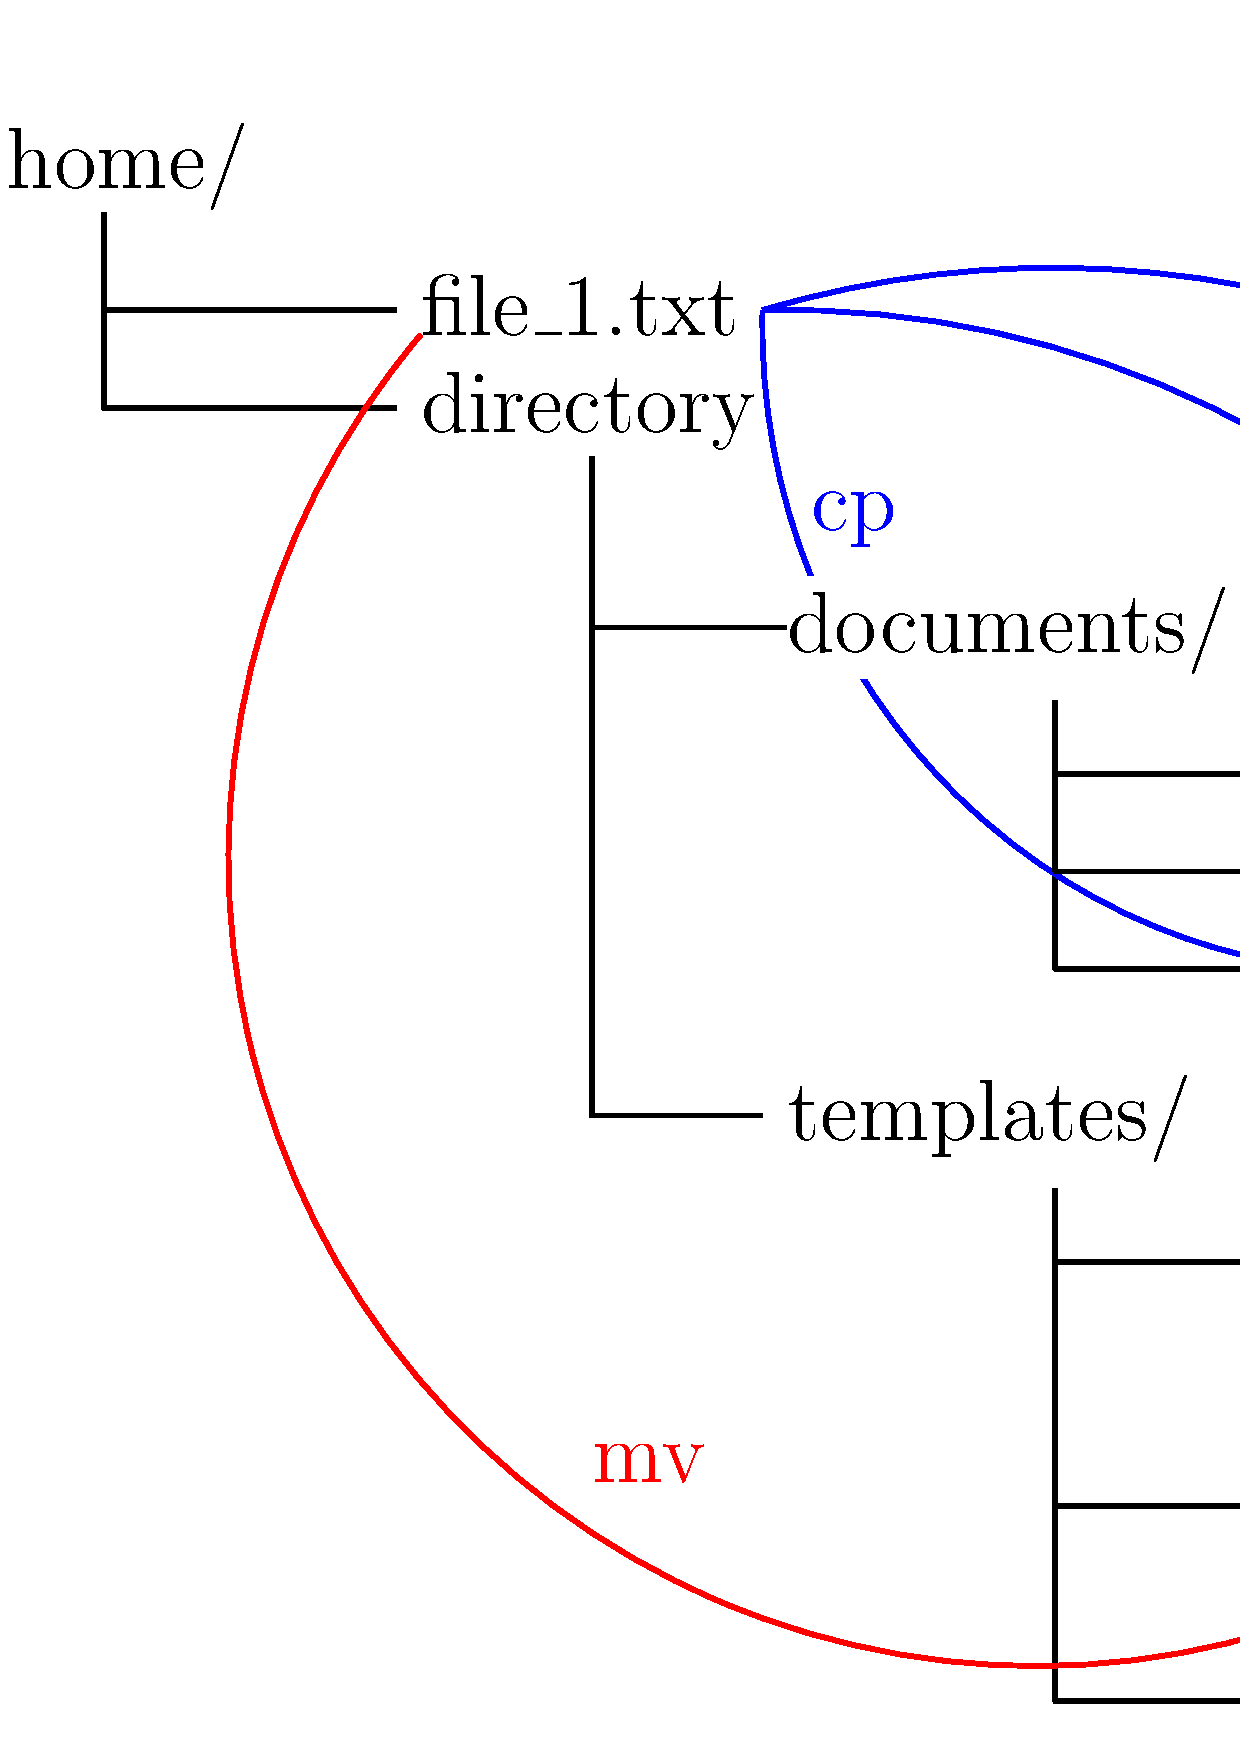
\includegraphics[width=0.80\textwidth]{pics/ex_2.png}
      \end{center}
    }

    \vspace{6mm}

    Create a script which filters out commented lines (starting with
    \code{\#}), selects all lines where the index is 2, then selects only who
    sells tamarindos. Use redirection and/or piping.

    \vspace{6mm}

    \focus{Hint}: the line begins with the index. Watch case.
    %grep -v '#' test | grep '^2 ' | grep -i 'tamarindo'
  \end{center}
\end{frame}

\begin{frame}
  \begin{center}
    \frametitle{Row Operations III - sed}

    \code{sed} (stream editor) operates on files as groups of lines:\\
    \focus{finds lines matching regexps and acts on (or around) them}

    \sidebyside{0.60}{
      \begin{itemize}
        \item \code{sed '/<regexp>/a <text>'}\\
          adds \code{<text>} after matching lines
        \item \code{sed '/<regexp>/i <text>'}\\
          adds \code{<text>} before matching lines
        \item \code{sed '/<regexp>/c <text>'}\\
          replaces matching lines with \code{<text>}
        \item \code{sed '/<regexp>/d'}\\
          deletes all matching lines
      \end{itemize}
    }{\hfill}{0.38}{
      \begin{center}
        \includegraphics[width=1.00\textwidth]{pics/sed-1.png}
      \end{center}
    }
  \end{center}
\end{frame}

\begin{frame}
  \begin{center}
    \frametitle{Row Operations IV - More sed}

     \code{sed 's/<regexp>/<text>/g' <files>}\\
     replaces \focus{all} occurrence of \code{<regexp>} with \code{<text>} in all lines

     \vspace{3mm}

     \sidebyside{0.54}{
       \begin{itemize}
         \item Replacement and matching\\
           will break words
         \item Matching is case-sensitive
         \item All regexp tools available
         \item \code{sed -i} applies modifications\\
           to the files: \focus{be careful!}
       \end{itemize}
     }{\hfill}{0.43}{
       \begin{center}
         \includegraphics[width=1.00\textwidth]{pics/sed-2.png}
       \end{center}
     }

     \vspace{3mm}

     Remember: \code{sed} can be used in pipes
  \end{center}
\end{frame}

\begin{frame}
  \begin{center}
    \frametitle{Exercise III - sed}

    \sidebyside{0.35}{
      Create the following file:
    }{\hfill}{0.60}{
      \begin{center}
        \includegraphics[width=0.70\textwidth]{pics/ex_3.png}
      \end{center}
    }

    \vspace{2mm}

    Create a script which:

    \begin{itemize}
      \item Replaces corrupted lines (lines containing \code{XXX}) with
        \code{\#CORRUPTED}
      \item Removes commented lines (beginning with \code{\#}) from the file
      \item Shows on screen the last two lines of the file replacing \code{,}
        with \code{.} (\focus{do not apply this last modification to the file})
    \end{itemize}

    \vspace{2mm}

    \focus{Hint:} the use of \code{sed -i} and pipes is suggested.\\
    A copy of the original file is also handy to have at all times.
  \end{center}
\end{frame}

\begin{frame}
  \begin{center}
    \frametitle{Column Operations I - cut and paste}

    Datafiles can also be seen as an ensemble of \focus{columns} (fields)

    \sidebyside{0.50}{
      \code{cut <options> <file>}:\\
      extract selected fields from file

      \vspace{3mm}

      \begin{itemize}
        \item \code{-d}: specify field delimiter\\
          (often \code{' '} or \code{','})
        \item \code{-f}: specify the desired fields\\
          (separate with \code{,})
        \item \code{--complement}:\\
          print unselected fields
      \end{itemize}
    }{\hfill}{0.46}{
      \begin{center}
        \includegraphics[width=1.00\textwidth]{pics/cut.png}
      \end{center}
    }

    \vspace{1mm}

    \sidebyside{0.49}{
      \code{paste <files>}:\\
      join lines in multiple files

      \begin{itemize}
        \item \code{-d}:\\
          specify delimiter between files\\
          default: \code{TAB} (not space!)
      \end{itemize}
    }{\hfill}{0.48}{
      \begin{center}
        \includegraphics[width=1.00\textwidth]{pics/paste.png}
      \end{center}
    }
  \end{center}
\end{frame}

\begin{frame}
  \begin{center}
    \frametitle{Column Operations II - sort}

    \sidebyside{0.62}{
      \code{sort <options> <file>}:\\
      \focus{sorts a file according to the given criteria}

      \vspace{4mm}

      \begin{itemize}
        \item \code{-k}: specify an index column\\
          (order following this column, default: 1)
        \item \code{-n}: numbers sorted according to value\\
        \item \code{-g}: like \code{-n}, more general formats\\
          (e.g., scientific notation)
        \item \code{-h}: like \code{-n}, human-readable formats\\
          (e.g., \code{4K, 8M})
        \item \code{-r}: reverses sort order (descending)
        \item \code{-u}: eliminates repeated lines
      \end{itemize}
    }{\hfill}{0.34}{
      \begin{center}
        \includegraphics[width=0.90\textwidth]{pics/sort.png}
      \end{center}
    }
  \end{center}
\end{frame}

\begin{frame}
  \begin{center}
    \frametitle{Exercise IV - cut, paste, sort}

    \sidebyside{0.35}{
      Create the following files:
    }{\hfill}{0.60}{
      \begin{center}
        \includegraphics[width=0.70\textwidth]{pics/ex_4.png}
      \end{center}
    }

    \vspace{3mm}

    Write a script which:

    \begin{itemize}
      \item Pastes the two files together
      \item Sorts the output according to the 3rd column
      \item Prints out the 2nd column of the line\\
        with the highest value of the 3rd column
    \end{itemize}

    \vspace{3mm}

    \focus{Hint}: Remember the options of \code{sort} (\code{-g} in
    particular).\\
    Remember \code{head/tail}.
  \end{center}
\end{frame}

\begin{frame}
  \begin{center}
    \frametitle{Column Operations III - awk}

    awk is a (simple) programming language for text operations\\
    mostly used to work on files as sets of columns

    \vspace{1mm}

    An awk program can be structured in 3 blocks:
    \code{BEGIN \{ 1 \} \{ 2 \} END \{ 3 \}}

    \vspace{1mm}

    \begin{itemize}
      \item \focus{Initial instructions} (1) are executed only once,\\
        before starting to read the file.
      \item \focus{Line instructions} (2) are executed on each line.
      \item \focus{Final instructions} (3) are executed once the file has been read.
    \end{itemize}

    \vspace{1mm}

    Usually when launched in shell only block (2) is used:\\
    \code{awk '\{ <commands> \}' <file>}

    \vspace{2mm}

    Powerful tools available, like \focus{if...then...else}\\
    We will not see them here (\focus{stackoverflow} is always there though)
  \end{center}
\end{frame}

\begin{frame}
  \begin{center}
    \frametitle{Column Operations IV - awk basics}

    \sidebyside{0.50}{
      \code{print} writes to standard output:\\
      use \code{""} for strings

      \vspace{4mm}

      Special variables:
      \begin{itemize}
        \item \code{NR} is the current line
        \item \code{NF} is the number of fields\\
          of the current line
      \end{itemize}
    }{\hfill}{0.45}{
      \begin{center}
        \includegraphics[width=0.75\textwidth]{pics/awk-1.png}
      \end{center}
    }

    \sidebyside{0.50}{
      Access fields via \code{\$<field\_number>}

      \begin{itemize}
        \item \code{\$0} is the entire line
        \item \code{\$NF} is the last field
      \end{itemize}

      \vspace{4mm}

      Fields can be manipulated\\
      as strings or floating-point numbers
      (file remains untouched)
    }{\hfill}{0.45}{
      \begin{center}
        \includegraphics[width=1.00\textwidth]{pics/awk-2.png}
      \end{center}
    }
  \end{center}
\end{frame}

\begin{frame}
  \begin{center}
    \frametitle{Exercise V - awk}

    \sidebyside{0.35}{
      Create the following file:
    }{\hfill}{0.60}{
      \begin{center}
        \includegraphics[width=0.70\textwidth]{pics/ex_5.png}
      \end{center}
    }

    \vspace{4mm}

    Write a script which writes to a new file the row number, the difference
    and the squared difference of columns 1 and 2 of the starting file
    (neglecting the label row).

    \vspace{4mm}

    In awk you can perform operations between columns,\\
    with the usual operators (\code{+, -, *, /, ()}).
  \end{center}
\end{frame}

\end{document}

%vim: tabstop=8 expandtab shiftwidth=2 softtabstop=2 spell spelllang=en_uk
